


In generale i sistemi di monitoraggio continuo di parametri fisiologici hanno bisogno di interfacciarsi con i sensori di interesse. 
Questo sistema non \`e una eccezione. 
Riteniamo che una interfaccia minima con lo stetoscopio elettronico sia quella illustrata nella figura \ref{interfacciastetoscopiominima}. Le operazioni illustrate sono:
\begin{description}
  \item[$connect$]
    Inizializza la connessione con il sensore ed allocare eventuali risorse necessarie.
  \item[$disconnect$]
    Terminare la connessione con il sensore e deallocare eventuali risorse.
  \item[$read$]
    Legge $length$ campioni di input e li memorizza nel buffer a partire dall'offset specificato.
  \item[$skip$]
    Tralascia un certo numero di campioni. Puo' essere utile per recuperare in parte un eventuale ritardo globale.
\end{description}



\begin{figure}
\centering
  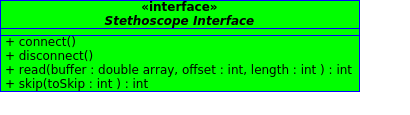
\includegraphics{./stethoscopeInterfaceOperations.png}
% stethoscopeInterfaceOperations.png: 410x115 pixel, 96dpi, 10.85x3.04 cm, bb=0 0 307 86
\caption{Operazioni dell'interfaccia con lo stetoscopio}
\label{interfacciastetoscopiominima}
\end{figure}



Il sistema deve includere almeno una componente che implementa l'interfaccia tra il dispositivo di monitoraggio e il sensore.
Alcune opzioni sono illustrate in figura \ref{componentiinterfacciastetoscopiominima}.

  \begin{figure}
  \centering
 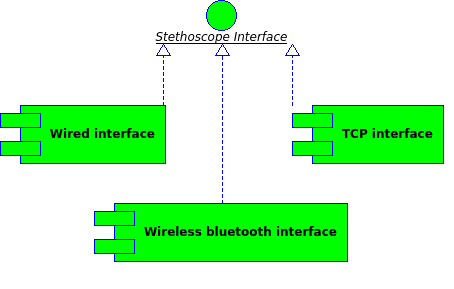
\includegraphics{./stethoscopeInterfaceComponent.png}
 % stethoscopeInterfaceComponent.png: 454x289 pixel, 96dpi, 12.01x7.65 cm, bb=0 0 340 217
  \caption{Possibili componenti che implementano l'interfaccia con lo stetoscopio}
  \label{componentiinterfacciastetoscopiominima}
  \end{figure}

Ci sono appunto vari modi di implementare una connessione tra lo stetoscopio e il dispositivo di monitoraggio. Una scelta che dobbiamo fare riguarda il mezzo di trasmissione del segnale:
\begin{description}
  \item[via cavo]
    In questa modalit\`a spesso \`e necessaria la presenza di personale medico specializzato. Tra gli svantaggi di questa impostazione notiamo: ridotta mobilit\`a del sistema, probabile necessit\`a di alimentazione elettrica dalla rete, rischio di gestione inadeguata di contatti nei cavi.
  \item[senza cavo]
    Una connessione senza fili presenta alcuni vantaggi ad esempio permette al paziente di muoversi pi\`u liberamente e i costi di installazione si possono ridurre.
\end{description}

Riteniamo che per questo sistema sia pi\`u adeguata una connessione senza fili. 

Un'altra scelta riguarda il protocollo di comunicazione, il quale per\`o potrebbe dipendere anche dalla scelta del mezzo di trasmissione.

% Streaming media is multimedia that is constantly received by and presented to an end-user while being delivered by a provider. Its verb form, "to stream", refers to the process of delivering media in this manner; the term refers to the delivery method of the medium rather than the medium itself.
% 
% A client media player can begin playing the data (such as a movie) before the entire file has been transmitted. Distinguishing delivery method from the media distributed applies specifically to telecommunications networks, as most other delivery systems are either inherently streaming (e.g., radio, television) or inherently nonstreaming (e.g., books, video cassettes, audio CDs). 
% For example, in the 1930s, muzak was among the earliest popularly available streaming media; nowadays Internet television is a common form of streamed media. 
% The term "streaming media" can apply to media other than video and audio such as live closed captioning, stock ticker, and real-time text, which are all considered "streaming text". 
% The term "streaming" was first used in the early 1990s as a better description for video on demand on IP networks; at the time such video was usually referred to as "store and forward video",[1] which was misleading nomenclature.
% 
% Live streaming, delivering live over the Internet, involves a camera for the media, an encoder to digitize the content, a media publisher, and a content delivery network to distribute and deliver the content.
% 
% 
% A broadband speed of 2.5 Mbit/s or more is recommended for streaming movies, for example to an Roku, Apple TV, Google TV or a Sony TV Blu-ray Disc Player, 10 Mbit/s for High Definition content.[8]
% 
% 
% 
% Unicast connections require multiple connections from the same streaming server even when it streams the same content
% Streaming media storage size is calculated from the streaming bandwidth and length of the media using the following formula (for a single user and file):
% 
% storage size (in megabytes) = length (in seconds) × bit rate (in bit/s) / (8 × 1024 × 1024)[note 1]
% Real world example:
% 
% One hour of video encoded at 300 kbit/s (this is a typical broadband video as of 2005 and it is usually encoded in a 320 × 240 pixels window size) will be:
% 
% (3,600 s × 300,000 bit/s) / (8×1024×1024) requires around 128 MB of storage.
% If the file is stored on a server for on-demand streaming and this stream is viewed by 1,000 people at the same time using a Unicast protocol, the requirement is:
% 
% 300 kbit/s × 1,000 = 300,000 kbit/s = 300 Mbit/s of bandwidth
% This is equivalent to around 135 GB per hour. Using a multicast protocol the server sends out only a single stream that is common to all users. 
% Therefore such a stream would only use 300 kbit/s of serving bandwidth. See below for more information on these protocols.
% 
% The calculation for live streaming is similar.
% 
% Assumptions: speed at the encoder, is 500 kbit/s.
% 
% If the show lasts for 3 hours with 3,000 viewers, then the calculation is:
% 
% Number of MBs transferred = encoder speed (in bit/s) × number of seconds × number of viewers / (8*1024*1024)
% Number of MBs transferred = 500 x 1024 (bit/s) × 3 × 3,600 ( = 3 hours) × 3,000 (nbr of viewers) / (8*1024*1024) = 1,977,539 MB





Siamo in presenza di un problema la cui modellazione porta naturalmente a pensare ad un pattern architetturale di tipo client server. 
Un server \`e un dispositivo fisico o virtuale che possiede una risorsa da condividere\cite{clientServer}, in questo caso il server \`e lo stetoscopio e la risorsa da condividere \`e il suono che esso registra. Un cliente \`e un dispositivo fisico o virtuale che richiede una certa risorsa ad un server\cite{clientServer}, in questo caso il client \`e il dispositivo di analisi del suono.



\paragraph{bluethoot}
In base alle considerazioni fatte da \cite{BBATMBS}, la teconologia wireless bluethoot si adatta bene al nostro sistema. Il bluethoot permette di stabilire semplici connessioni ad hoc tra dispositivi che hanno a disposizione poca energia elettrica e che sono posti a piccola distanza tra di loro, dove per piccola distanza approssimativamente intendiamo che i dispositivi si trovano nella stessa stanza o anche entro certi limiti in una stessa struttura ospedaliera. I valori precisi di consumi, distanze e velocit\`a di trasmissione variano da dispositivo a dispositivo. Lo stetoscopio elettronico invia continuamente dati al sistema di riconoscimento attraverso il canale bluethoot. I dati inviati dipendono dal particolare stetoscopio ma possiamo aspettarci che questi siano sotto forma di pacchetti di un segnale audio digitale. Suggeriamo quindi di implementare il sistema nel modo illustrato nella figura \ref{blueinterfacciastetoscopiominima}
\begin{figure}
 \centering
 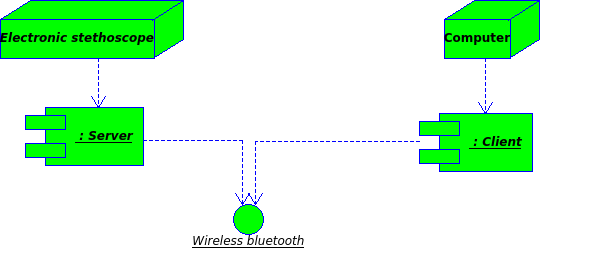
\includegraphics[width=0.9\textwidth]{./deploymentDiagram.png}
 % deploymentDiagram.png: 606x266 pixel, 96dpi, 16.03x7.04 cm, bb=0 0 454 199
  \caption{Architettura del sistema}
  \label{blueinterfacciastetoscopiominima}
\end{figure}


\paragraph{velocit\`a dell'intefaccia}

Supponiamo che il sistema abbia una velocit\`a media di esecuzione di $v_{s}$ campioni di segnale al secondo, e supponiamo che $v$ sia maggiore della frequenza di campionamento e che quindi il sistema riesca ad analizzare un segnale di un secondo in un tempo minore di un secondo. Questa velocit\`a si intende calcolata senza contare il tempo di trasmissione dallo stetoscopio al sistema.

Supponiamo che la velocit\`a di trasmissione dell'interfaccia tra sistema e stetoscopio sia $v_{i}$ bit al secondo e siano $f_{c}$ la frequenza di campionamento del segnale e $size$ la dimensione in bit di un campione di segnale. Allora deve valere
\[
  \displaystyle  \frac{f_{c}}{v_{s}} + \displaystyle \frac{f_{c}}{\left\lfloor\frac{v_{i}}{size}\right\rfloor} \leq 1s
\]
affinch\'e il sistema non accumuli ritardo.









